%==========================================
%
% SIBGRAPI 2018 paper
% Example of IEEEtran.cls, adapted for SIBGRAPI 2018 
%
%==========================================

% *** Authors should verify (and, if needed, correct) their LaTeX system  ***
% *** with the testflow diagnostic prior to trusting their LaTeX platform ***
% *** with production work. The IEEE's font choices and paper sizes can   ***
% *** trigger bugs that do not appear when using other class files.       ***                          ***
% The testflow support page is at:
% http://www.michaelshell.org/tex/testflow/

\documentclass[10pt,conference]{IEEEtran}

\usepackage{cite}

\ifCLASSINFOpdf
   \usepackage[pdftex]{graphicx}
   \graphicspath{{figs/}}
   \DeclareGraphicsExtensions{.pdf,.jpeg,.png}
\else
   \usepackage[dvips]{graphicx}
   \graphicspath{{../figs/}}
   \DeclareGraphicsExtensions{.eps}
\fi

\usepackage[cmex10]{amsmath}
\interdisplaylinepenalty=2500
\usepackage{amsthm}
\newtheorem{definition}{Definition}
\usepackage{algorithmic}
\usepackage{array}
\ifCLASSOPTIONcompsoc
  \usepackage[caption=false,font=normalsize,labelfont=sf,textfont=sf]{subfig}
\else
  \usepackage[caption=false,font=footnotesize]{subfig}
\fi
\usepackage{url}
\hyphenation{op-tical net-works semi-conduc-tor}


\begin{document}

\title{Scene Conversion for Physically-based Renderers}

\newif\iffinal
%\finalfalse
\finaltrue
\newcommand{\jemsid}{99999}
\iffinal

\author{\IEEEauthorblockN{Luiza Hagemann}
\IEEEauthorblockA{Instituto de Informática\\
Universidade Federal do Rio Grande do Sul\\
Porto Alegre, RS\\
lahagemann@inf.ufrgs.br}
\and
\IEEEauthorblockN{Manuel Menezes de Oliveira Neto}
\IEEEauthorblockA{Instituto de Informática\\
Universidade Federal do Rio Grande do Sul\\
Porto Alegre, RS\\
oliveira@inf.ufrgs.br}}

\else
  \author{SIBGRAPI paper ID: \jemsid \\ }
\fi

\maketitle

\begin{abstract}
The abstract goes here.
\end{abstract}

\IEEEpeerreviewmaketitle

\section{Introduction}

\section{Related Works}

\section{System Architecture}
Our converting pipeline is subdivided into three main states: the \textbf{Import 
Module}, the \textbf{Canonical Scene Representation} and the \textbf{Conversion 
Module}, as illustrated in Figure \ref{fig:sysarch}. Given an arbitrary input 
file format, our converter is able to import the scene and transform it into a 
generic, canonical representation and then export it to different output 
formats. 

\begin{figure}[h]
\centering
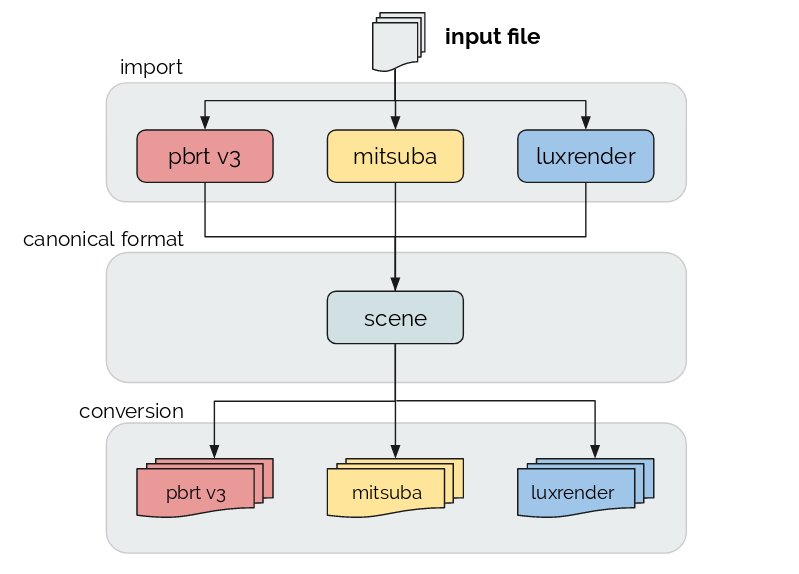
\includegraphics[width=2.5in]{figs/3_system_architecture/architecture.png}
\caption{Illustration of the system pipeline.}
\label{fig:sysarch}
\end{figure}

Our Proof of Concept encompassed \textit{PBRT} \cite{pbrt}, \textit{Mitsuba} 
\cite{mitsuba} and \textit{LuxRender} \cite{luxrender}, as these are three of 
the most popularly used renderers in the community.

\subsection{Import Module}
Most physically-based renderers have a similar way of describing a scene. 
Usually, they divide a scene into two sections: scene-wide rendering options and 
world block. The former defines overall rendering settings (such as which 
rendering or sampling technique should be used) while the latter describes the 
geometry and which materials should be used for rendering.

Our import module specializes in reading and interpreting such scene files. The 
input file is read, parsed and each directive is loaded into our canonical scene 
representation. Since each renderer has its own proprietary file format, we have 
three importing modules: one for each renderer.

\textit{PBRT} and \textit{LuxRender} file formats are composed of structured 
text statements defining all scene directives. Given their structure, a Lex/Yacc 
parser was considered the best choice for these formats. As we intended to keep 
our system in pure Python, we chose to use PLY \cite{ply}, a Python 
implementation of Lex and Yacc.

\textit{Mitsuba}'s file format consists of a XML file. Since there are several 
XML-parsing libraries for Python that can load the hierarchy into a tree data 
structure, we didn't think it necessary to create a Lex/Yacc parser. We chose to 
implement this module using ElementTree \cite{ET}, a XML parsing tool.

\subsection{Canonical Scene Representation}
After loading the scene file, the information obtained from them has to be 
stored somewhere. While most renderers have the same base structure, they differ 
in which parameters can be used to configure the techniques used during the 
rendering process. In order to establish a common ground for conversion, we 
defined a canonical scene representation. This representation can be easily 
extended incorporate any directives not contemplated in this work.

In this representation, we divide scene into the two sections stated in the 
section above: \textbf{scene-wide rendering options} and \textbf{world block}. 
The rendering options are divided into integration technique and sensor options, 
while the world block is divided into lists of shapes, global emitters and 
material definitions. This structure is illustrated in Figure 
\ref{fig:canonicalrep}.

\begin{figure}[h]
\centering
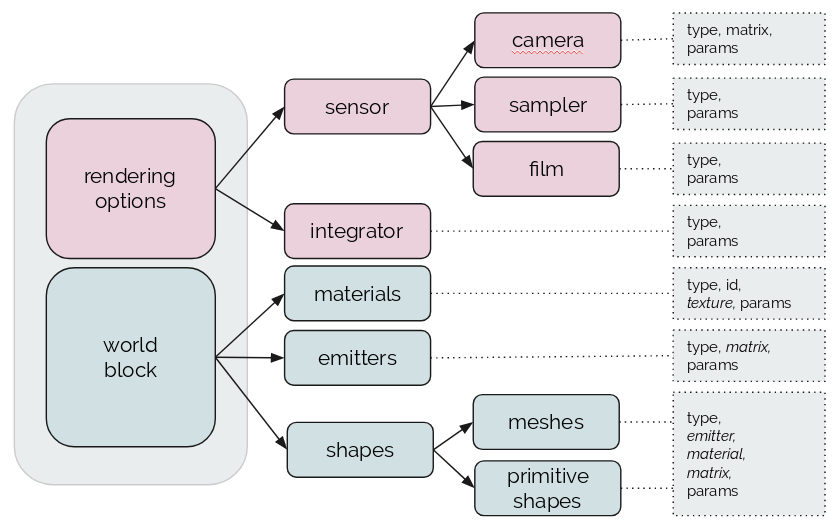
\includegraphics[width=2.5in]{figs/3_system_architecture/canonicalrep.png}
\caption{Illustration of the canonical scene representation.}
\label{fig:canonicalrep}
\end{figure}

\subsubsection{Scene-wide Rendering Options}
A set of directives specifying the integration and sampling techniques used for 
rendering, camera and film properties. These directives are represented in a 
structure with two fields: a \textbf{type} and a \textbf{list of parameters}.

\subsubsection{World Block}
A set of directives describing the shapes, materials and global emitters present in the scene. 

The shape directive is represented in a structure with: a \textbf{type} (cube, sphere, ...), an optional \textbf{area emitter}, an optional \textbf{material reference}, an optional \textbf{transformation matrix} and a \textbf{list of parameters}. 

The material directive is represented in a structure with: a \textbf{type}, an \textbf{id}, an optional \textbf{texture} and a \textbf{list of parameters}.

The global emitter directive is represented in a structure with: a \textbf{type}, an optional \textbf{transformation matrix} and a \textbf{list of parameters}.

\subsection{Conversion Module}
Subsection text here.

% An example of a floating figure using the graphicx package.
% Note that \label must occur AFTER (or within) \caption.
% \begin{figure}[!t]
% \centering
% 
\includegraphics[width=2.5in]{figs/SIBGRAPI2018-banner.png}
% % where an .eps filename suffix will be assumed under latex, 
% % and a .pdf suffix will be assumed for pdflatex; or what has been declared
% % via \DeclareGraphicsExtensions.
% \caption{SIBGRAPI - Conference on Graphics, Patterns and Images.}
% \label{fig_sim}
% \end{figure}

% An example of a double column floating figure using two subfigures.
% (The subfig.sty package must be loaded for this to work.)
% \begin{figure*}[!t]
% \centering
% \subfloat[Case I]{
\includegraphics[width=2.5in]{figs/SIBGRAPI2018-banner.png}%
% \label{fig_first_case}}
% \hfil
% \subfloat[Case II]{
\includegraphics[width=2.5in]{figs/SIBGRAPI2018-banner.png}%
% \label{fig_second_case}}
% \caption{SIBGRAPI - Conference on Graphics, Patterns and Images.}
% \label{fig_sim2}
% \end{figure*}
%

% An example of a floating table. Note that, for IEEE style tables, the
% \caption command should come BEFORE the table
% \begin{table}[]
% \renewcommand{\arraystretch}{1.3}
% \caption{An Example of a Table}
% \label{table_example}
% \centering
% \begin{tabular}{|c||c|}
% \hline
% One & Two\\
% \hline
% Three & Four\\
% \hline
% \end{tabular}
% \end{table}

\section{Results and Analysis}
Results section.

\section{Conclusion}
The conclusion goes here.

% conference papers do not normally have an appendix

% use section* for acknowledgment
\section*{Acknowledgment}


The authors would like to thank...

% trigger a \newpage just before the given reference
% number - used to balance the columns on the last page
% adjust value as needed - may need to be readjusted if
% the document is modified later
%\IEEEtriggeratref{8}
% The "triggered" command can be changed if desired:
%\IEEEtriggercmd{\enlargethispage{-5in}}

\bibliographystyle{IEEEtran}
\bibliography{example}
\end{document}


